% =====================================================================
\chapter{Le moteur de scénarios interactifs}
\label{ch:scenarios}
% =====================================================================

Un contrat JSON est difficile à vendre. Un souscripteur qui voit un JSON
comprend la donnée, mais il ne \emph{ressent} pas le risque. C'est la raison
d'être de la mise en situation sur la carte : rendre visible, sans mentir, ce
que le contrat décrit.

Ce chapitre raconte la construction de ce moteur — et les trois bugs
sémantiques qui ont dû être corrigés, chacun révélant une confusion
conceptuelle plus profonde qu'un simple défaut de code.

\section{Objectif et référence}

L'objectif est une boucle : choisir une classe de retour $\rightarrow$ l'eau
monte sur le bâtiment sur la carte ; déplacer un curseur horaire $\rightarrow$
le niveau évolue en direct ; appuyer sur \og Play \fg{} $\rightarrow$
l'animation se déroule jusqu'au pic.

La référence visuelle assumée est un projet de démonstration de visualisation
d'inondation (FuseLab), connu pour sa capacité à rendre une montée des eaux
lisible et crédible. L'enjeu était de reproduire cette lisibilité \emph{sans}
enfreindre les invariants du produit : aucune profondeur inventée, aucune
affirmation non étiquetée.

\begin{figure}[H]
\centering
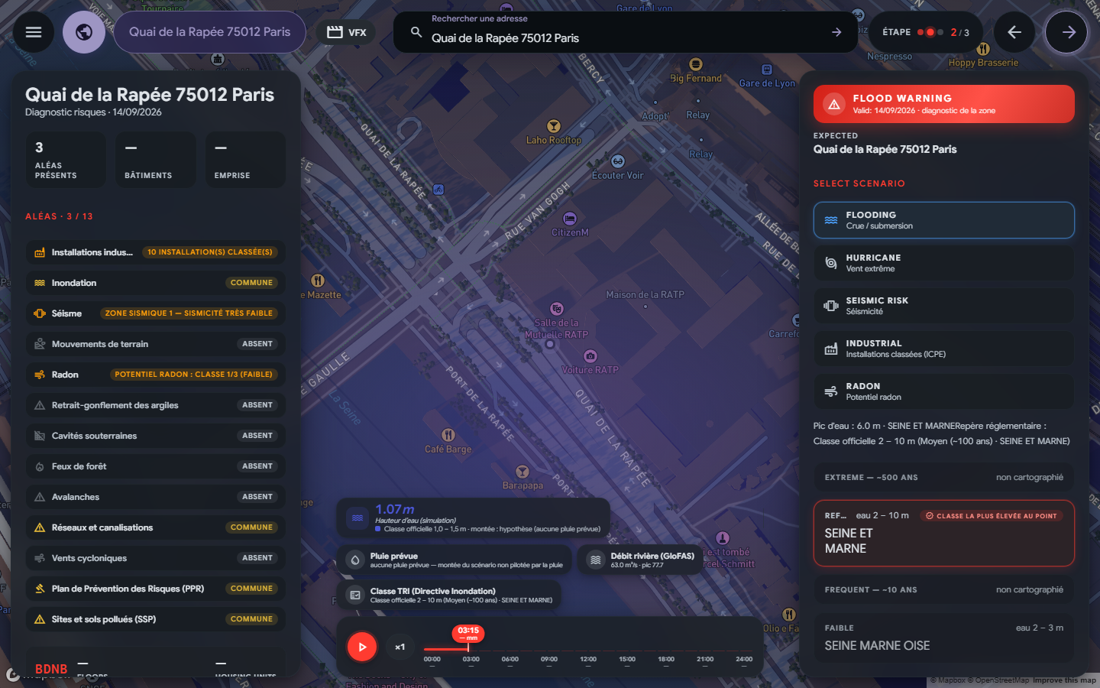
\includegraphics[width=0.92\textwidth]{../docs/screenshots/step2-scenario.png}
\caption{Étape 2 — simulation de scénario. À gauche, les classes TRI
officielles ; à droite, la timeline horaire et le bouton de lecture. L'eau
monte sur le bâtiment par extrusion Mapbox.}
\label{fig:step2}
\end{figure}

\section{Le bus d'état unique}

L'architecture repose sur un bus d'état minimal, partagé par la carte et les
panneaux :

\begin{center}
\code{scenarioKey} (classe TRI) \quad·\quad \code{hazardEvent} (aléa
sélectionné) \quad·\quad \code{riskTimeMin} (heure simulée)
\end{center}

Chaque aléa branche un rendu cartographique distinct — nappe d'eau, cône de
feu, couche de vent — mais tous lisent le même moteur. Aucun panneau ne
recalcule un niveau de façon indépendante : c'est la garantie que la console et
la carte affichent la même profondeur.

\begin{figure}[H]
\centering
\begin{tikzpicture}[
  scale=0.86, transform shape,
  node distance=5mm,
  innode/.style={draw=typhoonGrey!60,fill=typhoonSand,rounded corners=2pt,
             align=center,inner sep=4pt,font=\scriptsize,text width=2.3cm},
  st/.style={draw=typhoonBlue,fill=typhoonBlue!7,rounded corners=2pt,
             align=center,inner sep=4pt,font=\scriptsize,text width=2.3cm},
  eng/.style={draw=typhoonGreen,fill=typhoonGreen!8,rounded corners=2pt,
             align=center,inner sep=4pt,font=\scriptsize,text width=3.1cm},
  outnode/.style={draw=typhoonDeep,fill=typhoonDeep!8,rounded corners=2pt,
             align=center,inner sep=4pt,font=\scriptsize,text width=2.3cm},
  arrow/.style={-{Latex[length=1.8mm]},thick,typhoonBlue}
]
\node[innode] (tri) {Classes TRI\\{\tiny profondeur réglementaire}};
\node[innode,below=of tri] (rain) {Pluie horaire\\{\tiny Open-Meteo}};
\node[innode,below=of rain] (sk) {\code{scenarioKey}\\\code{riskTimeMin}};

\node[eng,right=10mm of rain] (eng) {\textbf{Moteur}\\
  \code{scenarioDepthAt}\\{\tiny le scénario fixe le pic,\\la pluie fixe la forme}};

\node[outnode,right=10mm of eng] (map) {Carte\\{\tiny extrusion d'eau}};
\node[outnode,above=of map] (cons) {Console\\{\tiny mêmes chiffres}};
\node[outnode,below=of map] (pan) {Panneau\\{\tiny vignettes honnêtes}};

\draw[arrow] (tri) -- (eng);
\draw[arrow] (rain) -- (eng);
\draw[arrow] (sk) -- (eng);
\draw[arrow] (eng) -- (map);
\draw[arrow] (eng) -- (cons);
\draw[arrow] (eng) -- (pan);
\end{tikzpicture}
\caption{Un seul bus d'état, un seul moteur. La carte et les panneaux ne
peuvent pas diverger.}
\label{fig:bus}
\end{figure}

\section{Bug 1 : les clés de scénario ne correspondaient pas}

\subsection{Symptôme}

Changer de scénario ne produisait rien : la carte restait sèche.

\subsection{Cause}

Le moteur utilisait des clés de scénario (\code{extreme}, \code{moyen},
\code{frequent}, \code{faible}) tandis que la couche d'interface utilisait une
autre table de correspondance (\code{direct}, \code{west}, \code{east},
\code{offshore}), vestige d'une première version où les scénarios étaient
géographiques. La fonction de résolution recevait donc une clé inconnue et
renvoyait \code{undefined}, silencieusement converti en \code{null} — donc
aucune eau.

\subsection{Correction}

Décision \scn{001} : \textbf{les clés du moteur \emph{sont} les clés
réglementaires TRI}. L'indirection est supprimée, ou réduite à un alias
documenté comme déprécié. Il n'existe plus qu'une seule source de vérité.

\section{Bug 2 : le seuil de dommages masquait la carte}

\subsection{Symptôme}

Même avec une clé correcte, la carte ne peignait rien avant un certain niveau.

\subsection{Cause}

Un seuil unique de 0,3~m servait à la fois à décider \og le bâtiment
subit-il des dommages ? \fg{} et \og faut-il peindre de l'eau sur la carte ? \fg.
Or une nappe de 0,1~m est un fait visuel réel, même si elle n'endommage pas
les équipements. Le seuil de dommages masquait la réalité physique.

\subsection{Correction}

Décision \scn{002} : \textbf{deux seuils, jamais confondus}. Le seuil de
0,3~m gouverne les dommages, les compteurs et les tuiles \og inondé \fg. La
carte, elle, peint dès que la profondeur dépasse une valeur plancher de 2~cm
(\code{MAP\_MIN\_DEPTH\_M}), en dessous de laquelle il ne reste qu'un résidu
numérique.

\begin{honesty}
Le seuil plancher de 2~cm est documenté explicitement : \og à t\textsubscript{0}
l'eau est visible \fg{} signifie \og au-delà de 2~cm \fg. C'est un détail, mais
c'est le genre de détail qui, non documenté, devient un rapport de bug
incompréhensible six mois plus tard.
\end{honesty}

\section{Bug 3 : \og rien ne se passe \fg{} par temps sec}

\subsection{Symptôme}

Sur une adresse réelle à Paris, après correction des deux bugs précédents, le
bouton de lecture restait inerte et changer de scénario ne produisait toujours
rien.

\subsection{Cause — deux causes distinctes}

L'investigation sur données réelles a montré deux problèmes indépendants.

\textbf{Cause A : le niveau dépendait de la météo du jour.} Le niveau d'eau
était calculé à partir de la prévision de pluie. Or ce jour-là à Paris, le
profil de pluie était vide (\code{dry: true}, cumul 0~mm) : la profondeur
valait donc 0 et le bouton était désactivé.

C'est une confusion conceptuelle : \emph{une classe de retour
réglementaire n'est pas une prévision météo}. La classe TRI \og 100 ans \fg{}
existe indépendamment du fait qu'il pleuve aujourd'hui.

\textbf{Cause B : la classe ouverte par défaut n'était pas cartographiée.} Le
scénario sélectionné par défaut était \code{extreme}, mais au point considéré
seule la classe \code{faible} était cartographiée. La résolution renvoyait
\code{null}, donc aucune eau.

\subsection{Corrections}

Décision \scn{004a} — \textbf{le scénario pilote le niveau, la pluie ne pilote
que la forme} :

\begin{center}
\code{scenarioDepthAt(profile, hourIndex, peakM)}
\end{center}

La classe TRI officielle fixe le pic — c'est un fait réglementaire. La
prévision de pluie ne fixe que la \emph{forme} de la courbe. En l'absence de
pluie, une rampe divergée documentée prend le relais et l'interface déclare
explicitement \og montée : hypothèse (aucune pluie prévue) \fg. L'ancienne
fonction dépendante de la météo reste exportée mais marquée dépréciée, avec
l'interdiction explicite de l'utiliser comme source du niveau.

Décision \scn{004b} — \textbf{sélection par défaut = classe la plus intense
réellement cartographiée}. Une fonction bascule sur la classe la plus intense
cartographiée, une seule fois par diagnostic, pour ne pas annuler un choix
explicite de l'utilisateur. Les classes non cartographiées deviennent
\code{disabled} avec une infobulle : un clic sans effet se lit comme un bug.

\begin{invariant}
Hors TRI ou absence de classe au point $\rightarrow$ strictement 0~m. Le pic
n'est \emph{jamais} deviné. La fonction \code{scenarioDepthAt} n'exagère que la
forme de la courbe, jamais son maximum.
\end{invariant}

\section{Le mode VFX et l'isolation des modes}

Un second mode de rendu, dit VFX, a été ajouté ultérieurement
(chapitre~\ref{ch:vfx}). Un point de conception important apparaît ici : le
mode VFX consomme \emph{le même} \code{scenarioDepthAt} que le mode données. Il
est donc impossible que les deux modes affichent deux hauteurs différentes.

De plus, lorsque le mode VFX est actif, la nappe d'eau du mode données est
explicitement désactivée (\code{impact=null}), ce qui évite deux nappes
superposées. Cette isolation est vérifiée par un test dédié.

\section{L'absence n'est pas une panne}

Un principe transversal mérite d'être isolé, car il a été formalisé comme
invariant (\scn{003}) : \textbf{l'absence d'un aléa et la panne d'un service
sont deux faits distincts}.

Le connecteur TRI porte cinq vérités différentes :

\begin{enumerate}[leftmargin=1.6em]
  \item chargement en cours ;
  \item service indisponible (panne) ;
  \item le point est dans un TRI mais aucune classe n'y est définie ;
  \item le point est hors TRI ;
  \item l'appartenance n'a pas pu être vérifiée.
\end{enumerate}

La formulation est \emph{partagée} entre le panneau, la console et le rapport :
une seule fonction produit le texte affiché. Cela évite le scénario classique
où trois composants décrivent le même état de trois façons légèrement
différentes, ce qui donne à l'utilisateur l'impression d'un système incohérent.

\begin{table}[H]
\centering
\small
\caption{Les messages distincts pour l'absence d'exposition.}
\label{tab:absence}
\begin{tabularx}{\textwidth}{@{}l X@{}}
\toprule
\textbf{Situation} & \textbf{Message} \\
\midrule
Hors TRI & \og Point non cartographié · Hors zone TRI \fg{} — un fait \\
\addlinespace
Dans un TRI, sans classe au point & Message distinct, sans chiffre — un fait
  réglementaire \\
\addlinespace
Service indisponible & \og Service indisponible · la cartographie TRI n'a pas
  répondu \fg{} — une panne \\
\bottomrule
\end{tabularx}
\end{table}

\section{Les autres aléas}

\subsection{L'ouragan}

En mode ouragan, l'eau est forcée à \code{null} — il n'y a pas d'inondation —
et une couche météorologique synchronisée à l'heure simulée affiche le vent et
la pluie. La console affiche la rafale et la bande correspondante.

\subsection{Le feu}

Pour l'aléa feu, un cône d'exposition est calculé à partir de la direction
réelle du vent et tracé sur la carte.

\begin{lstlisting}[caption={Construction du cône d'exposition au feu.},
label={lst:fire}]
fireConePolygon(meteo, originLonLat) -> GeoJSON Feature
  - cap     = provenance du vent + 180 degres
  - portee  = bornee par FIRE_REACH_MAX_KM = 1.5 km
  - ouverture heritee de fireConeFrom
\end{lstlisting}

Un écart assumé par rapport au plan initial mérite d'être signalé : la couche
devait être une extrusion 3D, elle a été réalisée en remplissage
(\code{fill}) et contour pointillé. La raison est explicite : \emph{un volume
3D sur un cône d'exposition suggérerait une précision qui n'existe pas}. Le
cône est une zone d'exposition possible, pas une emprise de flammes.

Le cône n'est monté que si l'aléa feu est sélectionné \emph{et} que le
diagnostic indique une exposition au feu. Sans météo, aucun cône n'est tracé et
un message explicite s'affiche.

\section{Synthèse des décisions du moteur}

\begin{table}[H]
\centering
\small
\caption{Décisions verrouillées du moteur de scénarios.}
\label{tab:scn}
\begin{tabularx}{\textwidth}{@{}l X@{}}
\toprule
\textbf{Décision} & \textbf{Contenu} \\
\midrule
\scn{001} & Les clés de scénario du moteur sont les clés réglementaires TRI.
  Pas de table de correspondance locale. \\
\addlinespace
\scn{002} & Deux seuils distincts : dommages (0,3~m) et carte (dès 2~cm). \\
\addlinespace
\scn{003} & Absence $\neq$ panne : cinq vérités distinctes, un texte partagé. \\
\addlinespace
\scn{004a} & Le scénario pilote le niveau, la pluie ne pilote que la forme. \\
\addlinespace
\scn{004b} & Sélection par défaut = classe la plus intense cartographiée,
  une fois par diagnostic. \\
\bottomrule
\end{tabularx}
\end{table}

Ces cinq décisions sont inscrites dans \fichier{AGENTS.md}, le document que
tout contributeur — humain ou agent — doit lire avant de modifier le code.
Chacune est accompagnée de la formulation \og ne jamais réintroduire \fg, avec
la raison historique. C'est la réponse méthodologique au problème posé au
chapitre~\ref{ch:methodo} : un correctif qui n'est pas documenté comme
invariant sera défait.
